\documentclass{beamer} % my version
\documentclass[handout]{beamer} % for audience
\usepackage{graphicx}
\usepackage{amsmath}
\usepackage{tcolorbox}
\usepackage{tikz}
\usetikzlibrary{positioning, arrows.meta, shapes.geometric}
% Center titles in beamer
\setbeamertemplate{frametitle}{\centering\insertframetitle}
% Title font customization for a bold look
\setbeamerfont{title}{size=\Large, series=\bfseries}
% Define custom environments
\newenvironment{mathmodel}{
    \begin{tcolorbox}[colback=violet!5, colframe=white, sharp corners, boxrule=0pt, title=Mathematical Model]
}{
    \end{tcolorbox}
}

\newenvironment{mathmod}{
    \begin{tcolorbox}[colback=blue!5, colframe=white, sharp corners, boxrule=0pt, title=Mathematical Model]
}{
    \end{tcolorbox}
}

\newenvironment{codebox}{
    \begin{tcolorbox}[colback=gray!10, colframe=black, sharp corners, boxrule=0.5pt, title=Code Box]
}{
    \end{tcolorbox}
}

% Define resized figures with smaller captions

\def\imgRepairChallenge#1{
    \refstepcounter{figure} % Increment figure counter
    \begin{center}
    \resizebox{\textwidth}{!}{ % Resize the entire figure to fit the frame width
    \begin{tikzpicture}[
        node distance=1.5cm, 
        process/.style={rectangle, draw, fill=orange!20, rounded corners, minimum height=2em, minimum width=3cm, text centered},
        repairpath/.style={rectangle, draw, fill=blue!10, rounded corners, minimum height=2em, minimum width=2.5cm, text centered},
        outcome/.style={rectangle, draw, fill=red!10, rounded corners, minimum height=2em, minimum width=2.5cm, text centered},
        hpath/.style={rectangle, draw, fill=green!10, rounded corners, minimum height=2em, minimum width=2.5cm, text centered},
        arrow/.style={thick, ->, >=Stealth}
    ]

    % Title Node
    \node[align=center, font=\large\bfseries, text width=8cm] at (0,2) {CRISPR/Cas9 DNA Repair Challenges};

    % Main Process Node - CRISPR Cut
    \node[process] (dsb) at (0,0) {CRISPR/Cas9 introduces a DSB};
    
    % Repair Pathways
    \node[repairpath, below left=0.8cm and 1.5cm of dsb] (nhej) {NHEJ Repair Pathway};
    \node[repairpath, below right=0.8cm and 1.5cm of dsb] (mmej) {MMEJ Repair Pathway};
    \node[hpath, below=0.8cm of dsb] (hdr) {HDR Repair Pathway};

    % Repair Outcomes
    \node[outcome, below=1.2cm of nhej] (nhej_outcome) {Random Indels (Insertions/Deletions)};
    \node[outcome, below=1.2cm of mmej] (mmej_outcome) {Predictable Small Deletions};
    \node[outcome, below=1.2cm of hdr] (hdr_outcome) {Template-Based Repair (Precise)};

    % Connections from DSB
    \draw[arrow] (dsb) -- node[above left] {Pathway 1} (nhej);
    \draw[arrow] (dsb) -- node[above right] {Pathway 2} (mmej);
    \draw[arrow] (dsb) -- node[right] {Pathway 3} (hdr);

    % Connections to Repair Outcomes
    \draw[arrow] (nhej) -- (nhej_outcome);
    \draw[arrow] (mmej) -- (mmej_outcome);
    \draw[arrow] (hdr) -- (hdr_outcome);

    % Additional Labels and Explanations
    \node[below=0.4cm of nhej_outcome, align=center, text width=3.5cm] {NHEJ is quick but\\ unpredictable};
    \node[below=0.4cm of mmej_outcome, align=center, text width=3.5cm] {MMEJ is predictable\\ but sequence-dependent};
    \node[below=0.4cm of hdr_outcome, align=center, text width=3.5cm] {HDR is precise but\\ requires a template};

    % Summary Explanation at Bottom
    \node[align=left,text width=18cm, below=6.5cm of dsb] {The challenge of CRISPR repair is that repair pathways like NHEJ and MMEJ can lead to unpredictable or variable outcomes, which complicates precise genome editing.};
    
    \node[align=right,text width=18cm, below=9cm of dsb] {\small Graph created with #1.};


    \end{tikzpicture}
    } % End of \resizebox
    \end{center}
    }

\def\imgInDelphiRelation#1{
    \refstepcounter{figure} % Increment figure counter
    \begin{center}
    \resizebox{\textwidth}{!}{
    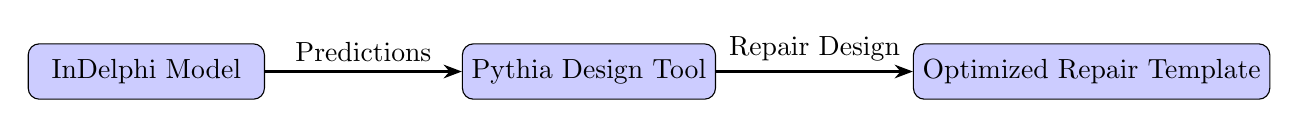
\begin{tikzpicture}[
        node distance=2.5cm,
        process/.style={rectangle, draw, fill=blue!20, rounded corners, text centered, minimum height=2em, minimum width=3cm},
        arrow/.style={thick, ->, >=Stealth}
    ]
    \node[process] (indelphi) {InDelphi Model};
    \node[process, right=of indelphi] (pythia) {Pythia Design Tool};
    \node[process, right=of pythia] (template) {Optimized Repair Template};

    \draw[arrow] (indelphi) -- node[anchor=south] {Predictions} (pythia);
    \draw[arrow] (pythia) -- node[anchor=south] {Repair Design} (template);
    \end{tikzpicture}
    }
    \end{center}
    \noindent\parbox[t]{0.48\textwidth}{\raggedright\small \textbf{Figure \thefigure}: #1}\\[1em]
}

\def\imgInDelphiLearning#1{
    \refstepcounter{figure} % Increment figure counter
    \begin{center}
    \resizebox{\textwidth}{!}{
    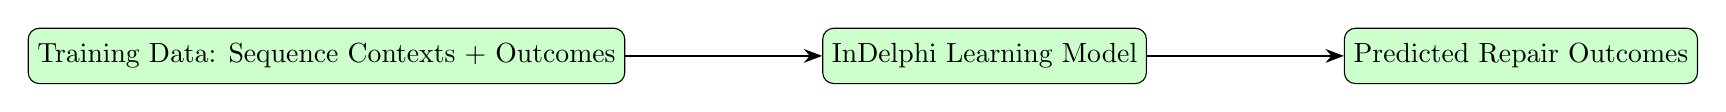
\begin{tikzpicture}[
        node distance=2.5cm,
        process/.style={rectangle, draw, fill=green!20, rounded corners, text centered, minimum height=2em, minimum width=3cm},
        arrow/.style={thick, ->, >=Stealth}
    ]
    \node[process] (input) {Training Data: Sequence Contexts + Outcomes};
    \node[process, right=of input] (model) {InDelphi Learning Model};
    \node[process, right=of model] (output) {Predicted Repair Outcomes};

    \draw[arrow] (input) -- (model);
    \draw[arrow] (model) -- (output);
    \end{tikzpicture}
    }
    \end{center}
    \noindent\parbox[t]{0.48\textwidth}{\small \textbf{Figure \thefigure}: #1}\\[1em]
}

\def\imgMMEJDiagram#1{
    \refstepcounter{figure} % Increment figure counter
    \begin{center}
    \begin{tikzpicture}[scale=0.8, transform shape]
        % DNA strand before the cut
        \draw[thick] (-4,0) -- (0,0); 
        
        % DSB site marked in red
        \fill[red] (-2, 0) circle (1.5pt); % Highlight DSB with a red dot
        \node[above] at (-2,0.2) {\textbf{\textcolor{red}{DSB}}};

        % Microhomology sequences marked in blue
        \draw[thick, dashed, blue] (-4, -0.8) -- (-1.5, -0.8); % Left microhomology
        \draw[thick, dashed, blue] (-1.5, -0.8) -- (0, -0.8); % Right microhomology
        \node[below] at (-3.75, -1.0) {\textbf{\textcolor{blue}{$\mu$Hs}}};
        \node[below] at (-0.25, -1.0) {\textbf{\textcolor{blue}{$\mu$Hs}}};

        % Deleted region marked in orange
        \draw[thick, orange] (-1.5, -0.8) -- (-2.5, -0.8); 
        \node[below] at (-2, -1.2) {\textbf{\textcolor{orange}{dels ($\Delta$)}}};

        % Title and explanation at the top and bottom
        \node[above=0.2cm of 2, align=center, font=\large\bfseries] {};
        \node[align=left, text width=12cm, below=3.5cm of 2] {\small Microhomologies (in blue) guide alignment at DSBs (in red), leading to predictable deletions (in orange) for more controlled editing.};
        \node[align=right, text width=10cm, below=6.5cm of 2] {\Small Graph created with Tikz.};

    \end{tikzpicture}
    \end{center}}

\def\imgPythiaTemplate#1{
    \refstepcounter{figure} % Increment figure counter
    \begin{center}
    \resizebox{\textwidth}{!}{
    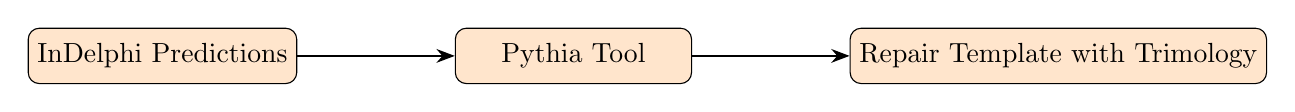
\begin{tikzpicture}[
        node distance=2cm,
        process/.style={rectangle, draw, fill=orange!20, rounded corners, text centered, minimum height=2em, minimum width=3cm},
        arrow/.style={thick, ->, >=Stealth}
    ]
    \node[process] (indelphi) {InDelphi Predictions};
    \node[process, right=of indelphi] (pythia) {Pythia Tool};
    \node[process, right=of pythia] (template) {Repair Template with Trimology};

    \draw[arrow] (indelphi) -- (pythia);
    \draw[arrow] (pythia) -- (template);
    \end{tikzpicture}
    }
    \end{center}
    \noindent\parbox[t]{0.48\textwidth}{\small \textbf{Figure \thefigure}: #1}\\[1em]
}

\title{InDelphi and Pythia in Genome Editing}
\author{Presented by: Hector Edu Nseng}
\date{\today}

\begin{document}

% Title Slide
\title{InDelphi and Pythia in Genome Editing}
\author{Presented by: [Your Name]}
\date{\today}

\begin{document}

% Title Slide
\begin{frame}
    \titlepage
\end{frame}

\begin{frame}{Introduction to CRISPR Repair Challenges}
  \only<beamer>{
  \begin{itemize}
      \item CRISPR/Cas9 creates double-strand breaks (DSBs) in DNA.
      \item Repair pathways  Non-Homologous End Joining (NHEJ), Microhomology-Mediated End Joining (MMEJ), Homology-Directed Repair (HDR) lead to varied outcomes, often unpredictable.
      \item Predictable repair is essential for precise gene editing applications.
  \end{itemize}
  \note{
      In this slide, introduce the concept of CRISPR creating DSBs. Mention that these breaks can be repaired through different pathways like NHEJ and MMEJ, leading to variable outcomes. This is a foundational challenge that *InDelphi* and *Pythia* aim to address.
    }
  }
  \only<handout>{
    {\imgRepairChallenge{PSTricks}}
    }
\end{frame}

% Slide 4: Microhomology-Mediated End Joining (MMEJ)
\begin{frame}{Microhomology-Mediated End Joining (MMEJ) (*explain*)}
  \only<handout>{
  \imgMMEJDiagram{}
  }
  % Updated Bullet Points with Emphasis on Color Coding
  \only<beamer>{
  \begin{itemize}
      \item MMEJ aligns DNA ends at a double-strand break (DSB) using short matching sequences called *microhomologies*.
      \item This alignment leads to the removal of non-matching sequences between microhomologies (orange), creating a small deletion in the repaired DNA.
  \end{itemize}
  }

\end{frame}



% Slide 1: Introduction to CRISPR Challenges (Presenter-Only Text)

\begin{frame}{Introduction to InDelphi’s Prediction Model (*explain*)}
  
  % Presenter Version: Bullet points only, no images
  \only<beamer>{
      \begin{itemize}
          \item *InDelphi* predicts gene editing outcomes by analyzing DNA sequence contexts around breaks. Here Cas9 introduces DSB...
          \item Microhomology sequences play a significant role in guiding deletion patterns. (panel a,b)
          \item Different DNA sequences lead to varied deletion profiles, showing the flexibility of *InDelphi*. (panel c)
      \end{itemize}
  }

  % Audience Version: Images only, no bullet points
  \only<handout>{
      \begin{figure}
        \raggedleft
          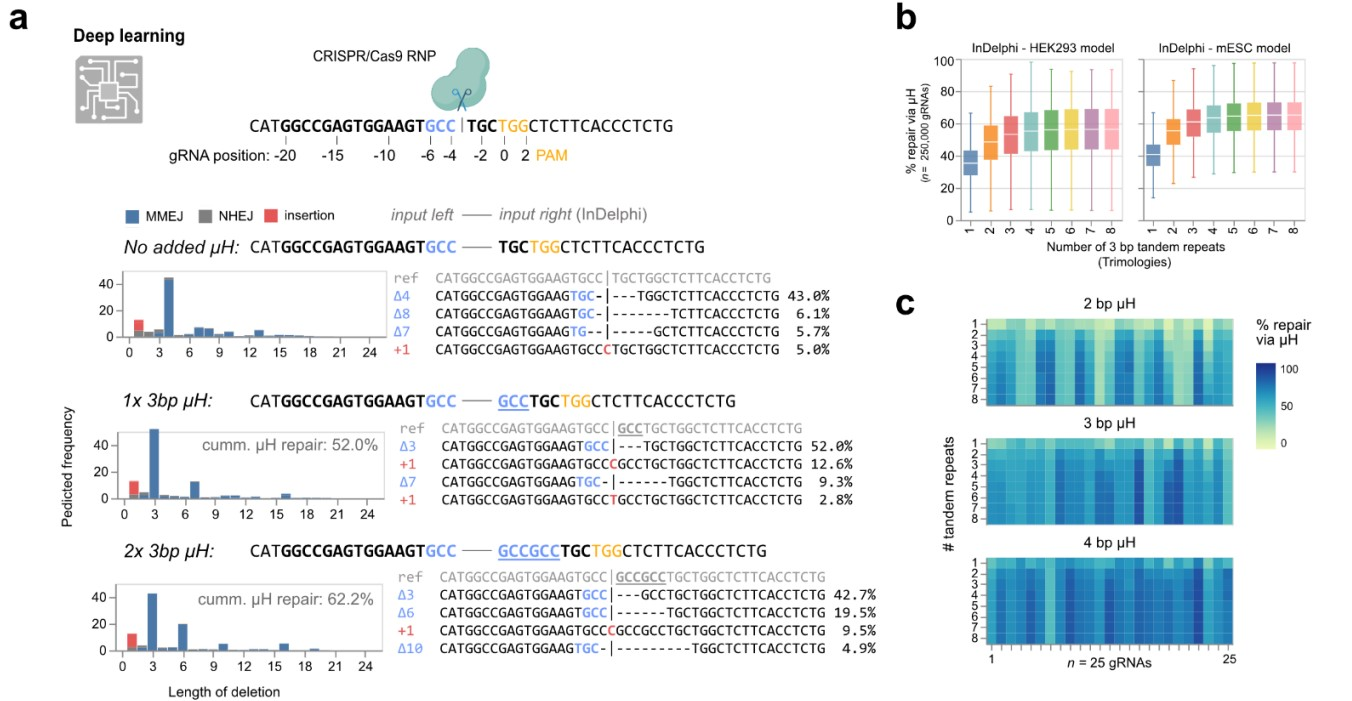
\includegraphics[width=1.1\textwidth]{fig/present/fig1_combined.jpeg}
          {\small \caption{\textit{InDelphi} model: predicted editing outcomes (a), role of microhomology in deletions (b), context-dependent deletion profiles (c).}}
        \end{figure}
  }

  % Presenter Notes
  \note{
      This slide introduces *InDelphi*'s predictive model. Discuss how it analyzes the DNA sequence around double-strand breaks to predict outcomes. 
      Emphasize the role of microhomology in influencing deletions, and explain how different DNA contexts lead to varied editing patterns, highlighting the model's adaptability.
  }
\end{frame}


\begin{frame}{Experimental Setup and Junction Analysis (*explain*)}
  % Presenter Version: Bullet points for explanation
  \only<beamer>{
      \begin{itemize}
          \item **Panel a**: Shows the design of the CRISPR/Cas9 strategy for inserting an eGFP gene using repair templates.
          \item **5' and 3' Junctions** (Panel g): 
            - Demonstrates real outcomes at both junctions, confirming deletions depend on microhomology (mH) usage.
          \item Each scaffold (1, 2, and 3) represents different configurations and the resulting sequence after repair.
      \end{itemize}
      \note{
          This slide highlights *Pythia*’s use of microhomology at integration junctions. Explain how CRISPR/Cas9 was used to deliver the eGFP gene, with the 5' and 3' junctions showing alignment using microhomology. Discuss how the presence of small deletions is consistent with MMEJ-based repair.
      }
  }

  % Audience Version: Image only
  \only<handout>{
      \begin{figure}
        \raggedright
          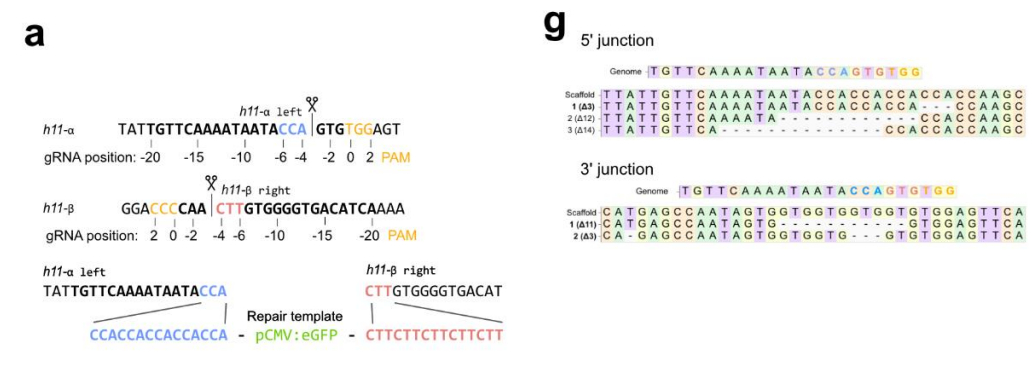
\includegraphics[width=\textwidth]{fig/present/fig3_1.jpeg}
          \caption{\small Experimental setup (a) and sequence analysis of 5' and 3' junctions (g), showing scaffold alignment and deletion patterns due to microhomology use.}
      \end{figure}
  }
\end{frame}

\begin{frame}{eGFP Expression in Xenopus Embryos}
  % Presenter Version: Bullet points for explanation
  \only<beamer>{
      \begin{itemize}
          \item **Figure b** Visualizes eGFP expression in various stages (neural, tadpole, forelimb).
          \item eGFP expression indicates successful integration of the repair template.
          \item Different levels and patterns of expression across developmental stages confirm successful integration into the genome.
      \end{itemize}
      \note{
          Describe how the eGFP marker helps visualize successful integration of the repair template. Explain that different stages (neural, tadpole, forelimb) provide insight into temporal and spatial expression, confirming that the editing process worked as intended.
      }
  }

  % Audience Version: Image only
  \only<handout>{
      \begin{figure}
          \centering
          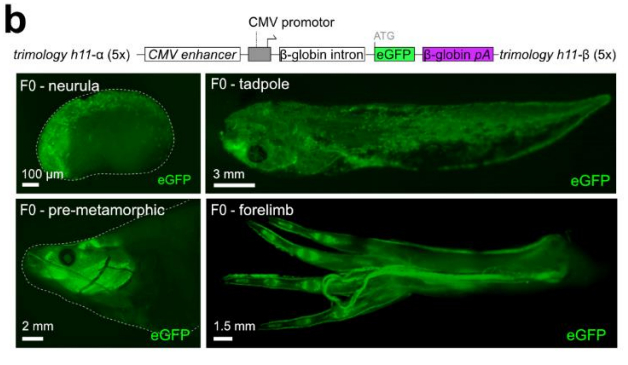
\includegraphics[width=\textwidth]{fig/present/fig3_2.jpeg}
          \caption{\small Expression of eGFP in \textit{Xenopus} at various developmental stages, demonstrating successful integration.}
      \end{figure}
  }
\end{frame}
\begin{frame}{eGFP and dsRed2 Expression Validation in F2 Generation}
  % Presenter Version: Bullet points for explanation
  \only<beamer>{
      \begin{itemize}
          \item **Panel j** Shows eGFP expression in F2 tadpole kidney, confirming inheritance of the transgene.
          \item **Panel k-l** Visualizes dsRed2 expression in muscle tissue of F2 homozygote, showing stable integration and expression in F2 offspring.
          \item This confirms that the genome edits are heritable, supporting *Pythia*’s efficacy in generating inheritable modifications.
      \end{itemize}
      \note{
          Explain the significance of eGFP and dsRed2 expression in the F2 generation, indicating successful germline transmission. Emphasize that these results validate *Pythia*’s predictions not only for targeted tissue expression but also for inheritable genomic modifications, which is essential for applications requiring stable gene integration across generations.
      }
  }

  % Audience Version: Image only
  \only<handout>{
      \begin{figure}
          \centering
          \hspace{-3em} % Shift the image slightly to the left
          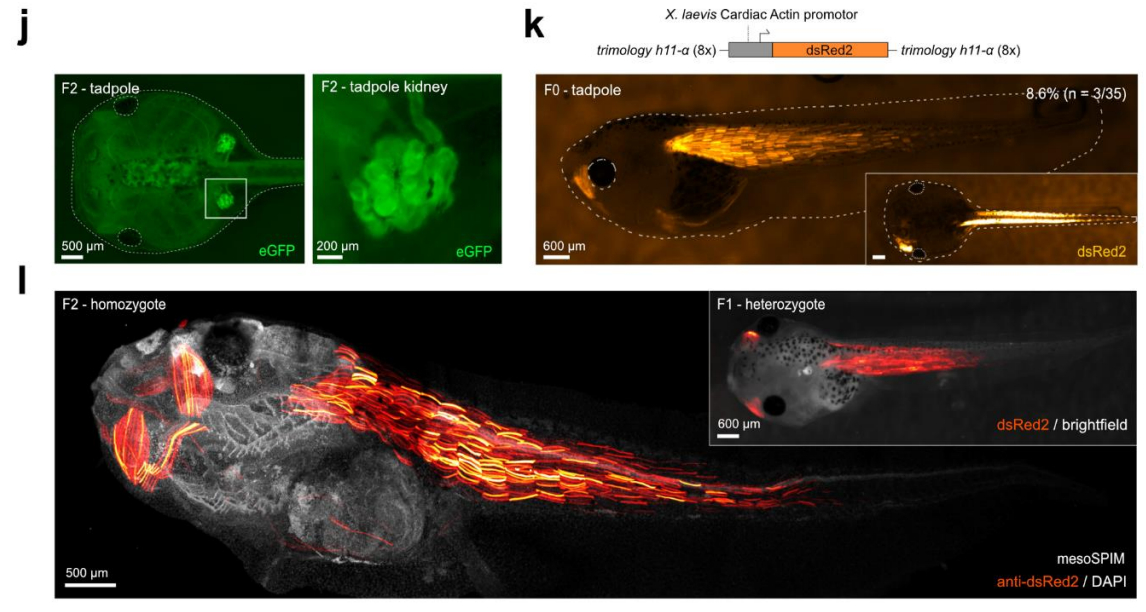
\includegraphics[width=\textwidth]{fig/present/fig3_3.jpeg}
          \caption{\small eGFP and dsRed2 expression in F2 generation, validating inheritable integration across tissues and developmental stages in \textit{Xenopus} embryos.}
      \end{figure}
  }
\end{frame}
\begin{frame}{In vivo Genome Editing in Neuronal Cells: Experimental Setup (*explain*)}
  % Presenter Version: Bullet points for explanation
  \only<beamer>{
      \begin{itemize}
        \item **Panel e,f** shows the repair template design targeting the Tubb2a gene, using trimology sequences to predict specific deletions (Δ3, Δ6, Δ9) in Tubb2a.
          \item **panel a** shows Design strategy using *Pythia* to target the Tubb2a gene with CRISPR/Cas9 and repair templates.
          \item **panel b**: Injection setup in mouse brain regions (V1 and hippocampus) for precise targeting.
      \end{itemize}
      \note{
          Describe the design of the CRISPR/Cas9 strategy for targeting Tubb2a in mouse brain cells, including the use of trimology-based repair templates. Explain the brain injection setup and how tissue staining with mCherry and GFP confirms localization at the target sites (V1 and hippocampus).
      }
  }

  % Audience Version: Image only
  \only<handout>{
      \begin{figure}
          \centering
          \hspace{-3em} % Move the image slightly to the left if needed
          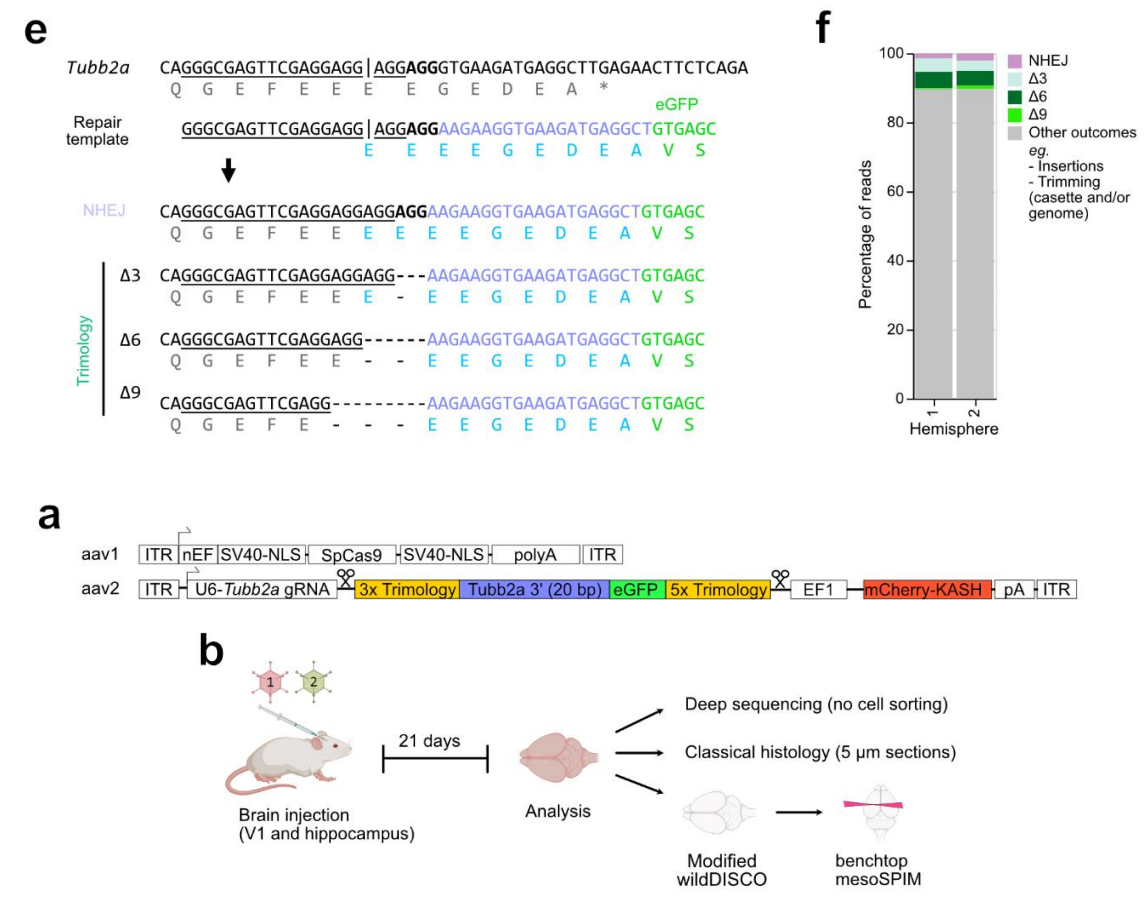
\includegraphics[width=0.7\textwidth]{fig/present/fig4_1.jpeg} % First part of Figure 4
          \caption{\small CRISPR/Cas9 design for Tubb2a targeting (a), injection setup in brain regions (b), \textit{trimology} sequence and predicted deletions (Δ3, Δ6, Δ9)(4e,f).}
      \end{figure}
  }
\end{frame}

\begin{frame}{Repair Outcomes and Neuronal Localization}
  % Presenter Version: Bullet points for explanation
  \only<beamer>{
    \begin{itemize}
      \item The figure shows Efficiency of repair across both brain hemispheres, demonstrating reliable on-target editing.
      \item The high-resolution images also confirm successful localization of edits within cortical and hippocampal neurons.
  \end{itemize}      
  \note{
          Discuss the experimental outcomes shown in Figure e, where trimology-based repair generates specific small deletions in the Tubb2a gene. Highlight the high efficiency of repair (4f) across brain hemispheres. Use Figures g and h to illustrate the precise localization of edits in cortical and hippocampal neurons, confirming Pythia’s specificity and precision.
      }
  }

  % Audience Version: Image only
  \only<handout>{
      \begin{figure}
          \centering
          \hspace{-3em} % Move the image slightly to the left if needed
          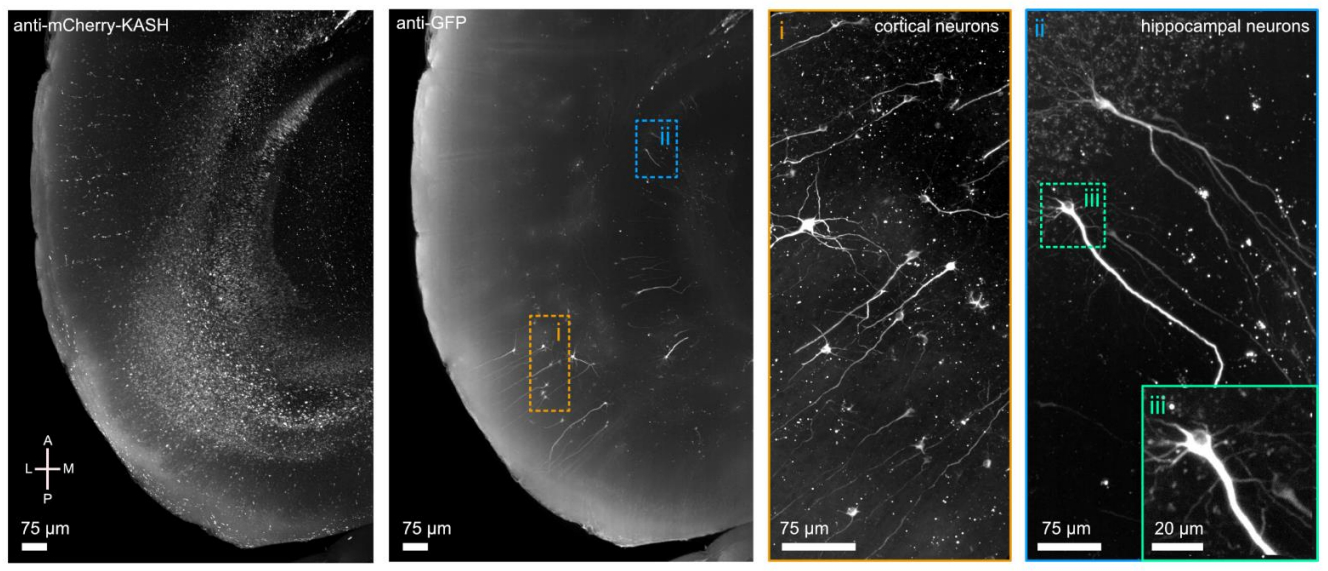
\includegraphics[width=\textwidth]{fig/present/fig4_2.jpeg} % Second part of Figure 4
          \caption{\small Trimology-based repair outcomes (e, f) and high-resolution neuronal localization (g, h), confirming precision in cortical and hippocampal neurons.}
      \end{figure}
  }
\end{frame}

\begin{frame}{Deep Learning Prediction Model for Single Nucleotide Edits (*explain*)}
  % Presenter Version: Bullet points for explanation
  \only<beamer>{
      \begin{itemize}
          \item The Pythia model also uses its deep learning model to predict and design single nucleotide edits, here the authors Demonstrate the convertion of eGFP to eBFP.
          \item Deep learning selects optimal gRNAs and repair template designs based on SNP location. (*explain*)
          \item the scoring system for repair arms, optimizes the edit based on predicted left and right junction outcomes. (*Explain*)
          \item So, the Pythia matrix helps us find the optimal length for the repair arms.
      \end{itemize}
      \note{
          Explain how Pythia uses a deep learning approach to predict and design single nucleotide edits, such as converting eGFP to eBFP. Emphasize the scoring system for repair arms, which optimizes the edit based on predicted left and right junction outcomes.
      }
  }

  % Audience Version: Image only
  \only<handout>{
      \begin{figure}
          \centering
          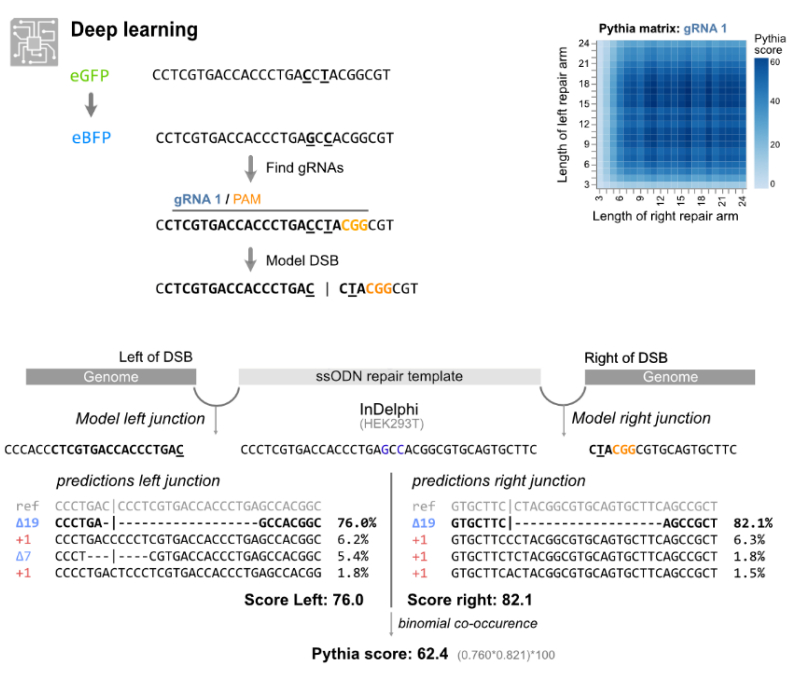
\includegraphics[width=0.7\textwidth]{fig/present/fig5_1.jpeg} % Replace with the path to fig5_1.jpeg
          \caption{\small Prediction model for single nucleotide editing to convert eGFP to eBFP, using deep learning to guide template design.}
      \end{figure}
  }
\end{frame}

\begin{frame}{Experimental Validation for Single Nucleotide Editing (*explain*)}
  % Presenter Version: Bullet points for explanation
  \only<beamer>{
      \begin{itemize}
          \item This eGFP to eBFP conversion was demonstrated Experimentally.
          \item The predicted deep learning model for the conversion of GFP to BFG was implemented comparing three different Pythia scores. 
          \item The SNP-based conversion was then confirmed through flow cytometry, aligning with Pythia’s high prediction scores.
          \item Higher Pythia scores are associated with greater SNP conversion efficiency.
      \end{itemize}
      \note{
          Describe the experimental validation setup where Pythia predictions for single nucleotide edits are tested by converting eGFP to eBFP. Flow cytometry results show that higher Pythia scores lead to higher editing efficiency, confirming the accuracy of predictions.
      }
  }

  % Audience Version: Image only
  \only<handout>{
      \begin{figure}
          \centering
          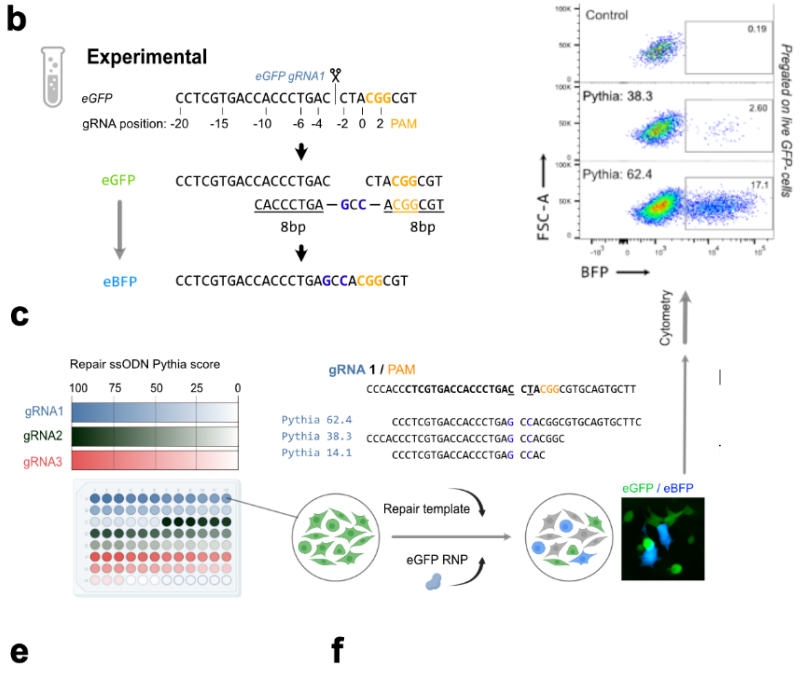
\includegraphics[width=0.7\textwidth]{fig/present/fig5_2.jpeg} % Replace with the path to fig5_2.jpeg
          \caption{\small Experimental validation of single nucleotide conversion (eGFP to eBFP) using Pythia’s optimized templates and flow cytometry analysis.}
      \end{figure}
  }
\end{frame}
\begin{frame}{Correlation of Pythia Scores with SNP Editing Efficiency (*explain-quick*)}
  % Presenter Version: Bullet points for explanation
  \only<beamer>{
      \begin{itemize}
          \item Scatter plot also confirmed a significant correlation between Pythia scores and successful SNP conversion rates (panel d).
          \item Which means that higher Pythia scores correlate strongly with higher conversion efficiencies for precise SNP editing (panel e)
          \item This finding validated Pythia’s reliability for predicting SNP editing outcomes.
      \end{itemize}
      \note{
          Highlight the correlation between Pythia scores and editing efficiency shown in Figure d. Explain that a higher Pythia score aligns with higher SNP conversion rates, validating Pythia’s accuracy for single nucleotide predictions.
      }
  }

  % Audience Version: Image only
  \only<handout>{
      \begin{figure}
          \centering
          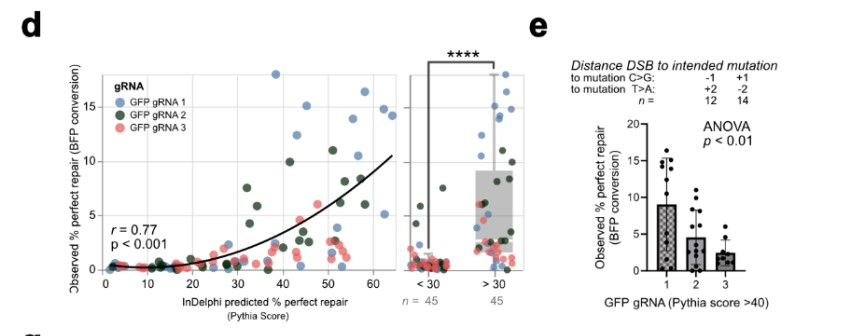
\includegraphics[width=1\textwidth]{fig/present/fig5_3.jpeg} % Replace with the path to fig5_3.jpeg
          \caption{\small Correlation between Pythia scores and successful SNP conversion rates, supporting predictive accuracy.}
      \end{figure}
  }
\end{frame}
\begin{frame}{Clinical Application for SNP Corrections in RPE65 Gene Therapy (*explain*-quick)}
  % Presenter Version: Bullet points for explanation
  \only<beamer>{
      \begin{itemize}
          \item The authors also applied Pythia on to the RPE65 gene for single nucleotide mutation correction.
          \item The Pythia scores identified optimal repair arm lengths to maximize editing accuracy.
          \item This demonstrated Pythia’s potential for potential for designing precise therapeutic templates for single nucleotide corrections in clinical gene therapy.
      \end{itemize}
      \note{
          Describe how Pythia applies to the RPE65 gene to guide SNP corrections associated with genetic conditions like Leber congenital amaurosis. Emphasize the tool’s potential for designing precise therapeutic templates for single nucleotide corrections.
      }
  }

  % Audience Version: Image only
  \only<handout>{
      \begin{figure}
          \centering
          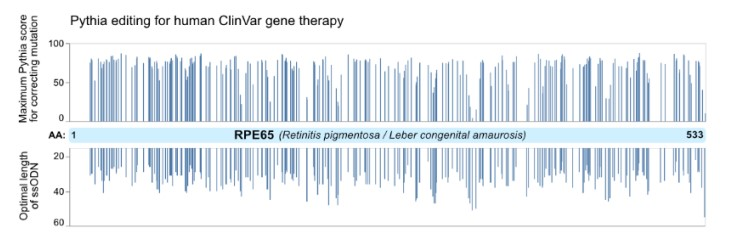
\includegraphics[width=1.1\textwidth]{fig/present/fig5_4.jpeg} % Replace with the path to fig5_4.jpeg
          \caption{\small Clinical application of Pythia for precise SNP corrections in RPE65 gene therapy, relevant to Leber congenital amaurosis.}
      \end{figure}
  }
\end{frame}
% Conclusion Slide
\begin{frame}{Conclusion}
  \begin{itemize}
      \item \textbf{Precision in CRISPR Editing}
          \begin{itemize}
              \item InDelphi + Pythia enable controlled, predictable edits
              \item Effective near microhomology regions for guided repairs
          \end{itemize}
      
      \item \textbf{Clinical Suitability}
          \begin{itemize}
              \item Suitable for single-gene corrections with accessible PAM sites
              \item Challenges: Complexity in repetitive regions, off-target risks
          \end{itemize}
      
      \item \textbf{Key Applications}
          \begin{itemize}
              \item Therapeutic gene editing (e.g., RPE65-related diseases)
              \item High-fidelity gene tagging in research
              \item Improved precision in gene drive systems
          \end{itemize}
  \end{itemize}
\end{frame}
% Thank You Slide
\begin{frame}
  \centering
  \Huge{Thank You!}
\end{frame}
\end{document}
